\documentclass{sigchi}

% Use this command to override the default ACM copyright statement (e.g. for preprints). 
% Consult the conference website for the camera-ready copyright statement.
\toappear{
	Submitted for review.
}

% Arabic page numbers for submission. 
% Remove this line to eliminate page numbers for the camera ready copy
\pagenumbering{arabic}


% Load basic packages
\usepackage{balance}  % to better equalize the last page
\usepackage{graphics} % for EPS, load graphicx instead
\usepackage{times}    % comment if you want LaTeX's default font
\usepackage{url}      % llt: nicely formatted URLs

\usepackage{textcomp}


% llt: Define a global style for URLs, rather that the default one
\makeatletter
\def\url@leostyle{%
  \@ifundefined{selectfont}{\def\UrlFont{\sf}}{\def\UrlFont{\small\bf\ttfamily}}}
\makeatother
\urlstyle{leo}


% To make various LaTeX processors do the right thing with page size.
\def\pprw{8.5in}
\def\pprh{11in}
\special{papersize=\pprw,\pprh}
\setlength{\paperwidth}{\pprw}
\setlength{\paperheight}{\pprh}
\setlength{\pdfpagewidth}{\pprw}
\setlength{\pdfpageheight}{\pprh}

% Make sure hyperref comes last of your loaded packages, 
% to give it a fighting chance of not being over-written, 
% since its job is to redefine many LaTeX commands.
\usepackage[pdftex]{hyperref}
\hypersetup{
pdftitle={Augmented Reality Tools for 
  the Creation of Physical Visual Arts},
pdfauthor={LaTeX},
pdfkeywords={mixed reality, projection mapping, drawing, touch input},
bookmarksnumbered,
pdfstartview={FitH},
colorlinks,
citecolor=black,
filecolor=black,
linkcolor=black,
urlcolor=black,
breaklinks=true,
}

% create a shortcut to typeset table headings
\newcommand\tabhead[1]{\small\textbf{#1}}

% End of preamble. Here it comes the document.
\begin{document}

\title{Mixed drawing - merging traditional and digital drawing}

%\numberofauthors{1}
%\author{
%  \alignauthor 1st Author Name\\
%    \affaddr{Affiliation}\\
%    \affaddr{Address}\\
%    \email{e-mail address}\\
%}

 \numberofauthors{2}
 \author{
   \alignauthor 1st Author Name\\
     \affaddr{Affiliation}\\
     \affaddr{Address}\\
     \email{e-mail address}\\
   \alignauthor 2nd Author Name\\
     \affaddr{Affiliation}\\
     \affaddr{Address}\\
     \email{e-mail address}\\
 }



%% \begin{figure*}[th]
%% \centering
%% 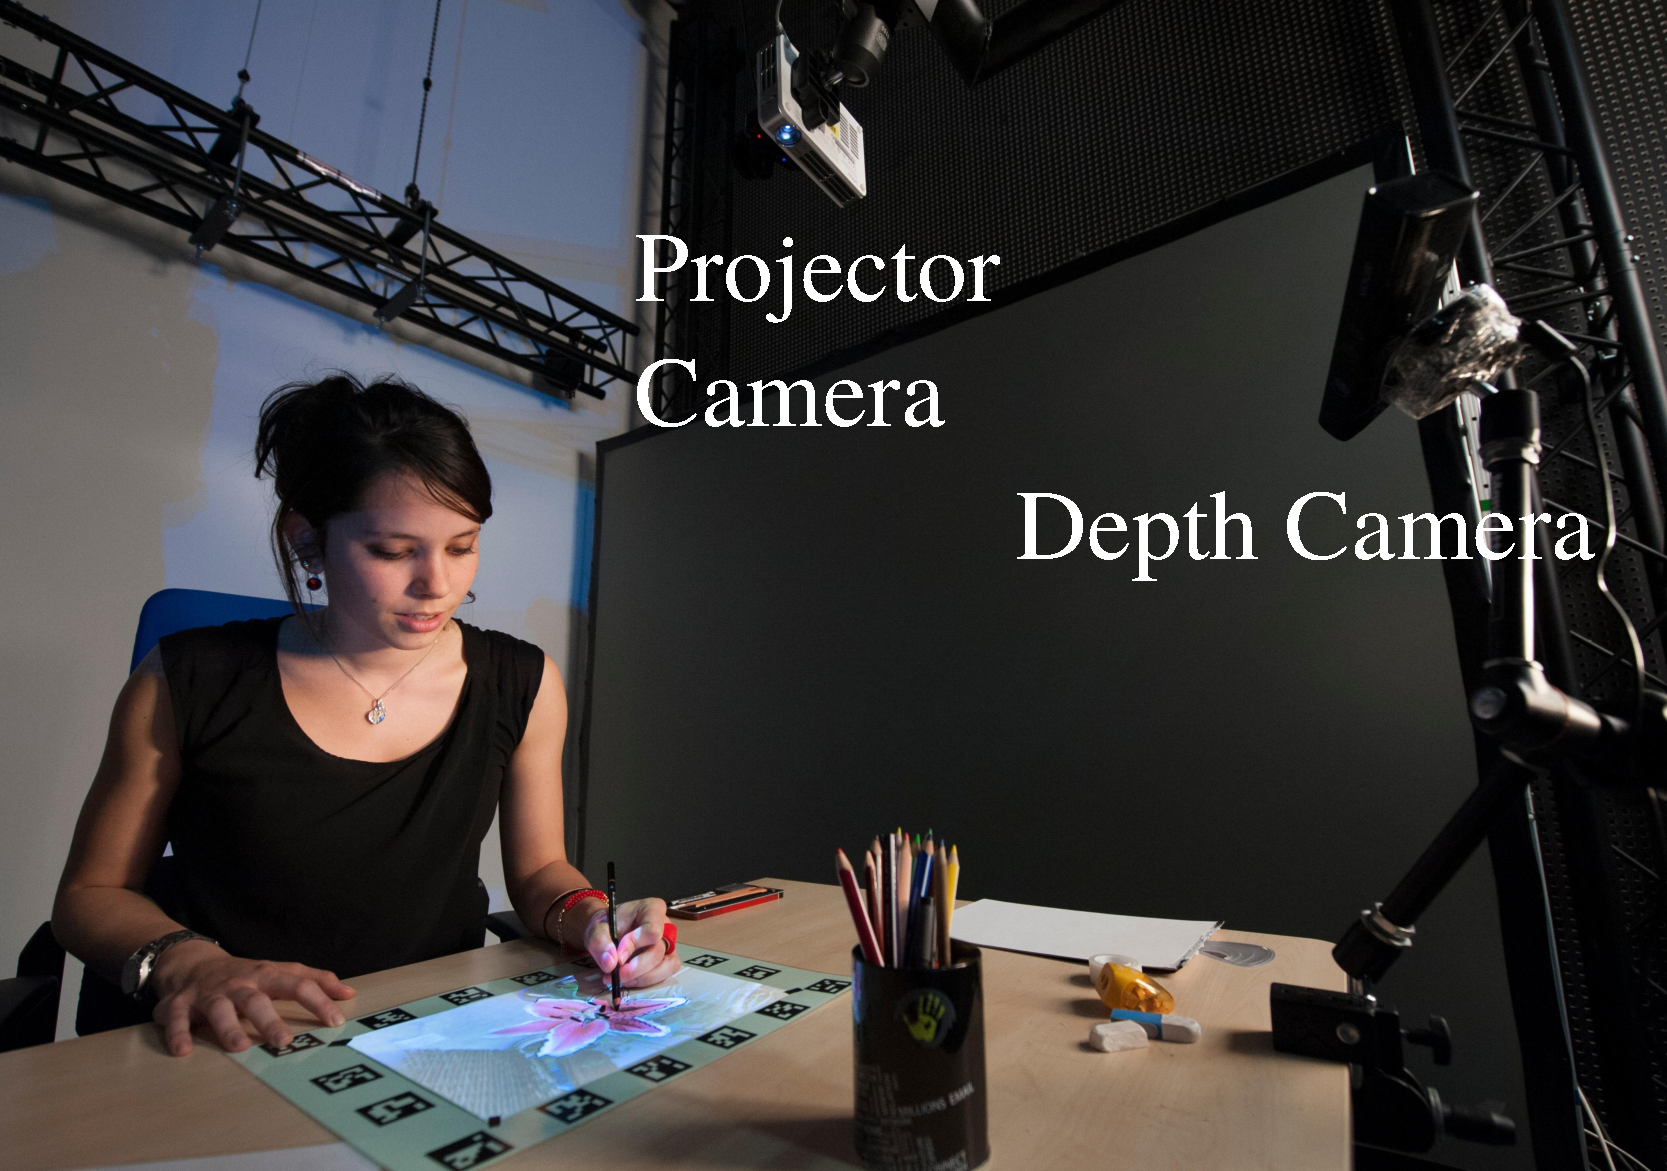
\includegraphics[width=85mm]{systempro.pdf}
%% \caption{Projection mapping resulting system.}
%% \label{fig:teaser}
%% \end{figure*}





\maketitle
 

%\vspace{55mm}
%
\includegraphics[height=55mm]{teaser.pdf}

\begin{abstract}

\end{abstract}


\keywords{mixed reality, projection mapping, drawing, touch input}
% \vspace{-0.15cm}


\category{H.5.1}{Information interfaces and presentation}{Information interfaces and presentation}
% \vspace{-0.15cm}

\terms{Design, Human Factors}
% \vspace{-0.15cm}

%% \keywords{
%% 	augmented reality; projection mapping; drawing; painting; non
%%         photorealistic rendering
%% }



\section{Introduction}
\begin{itemize}
	\item Motivation
	\item General approach 
\end{itemize}


\section{Pevious work}


\section{Technical setup}
\begin{itemize}
	\item SAR - markers, projection  (main paper + additional cardboards)
	\item Touch - Kinect
	\item Capture - additional Camera	 
	\item Processing
\end{itemize}


\section{Digital tools for traditional drawing}

\subsection{Interacting with a projected image}
\begin{itemize}
  \item projection of an image in the canvas (choose the good position to trace the projected image)
	\item modification of the display (RST mutitouch gesture) + transparency		 
\end{itemize}

\subsection{Compositing the image}
\begin{itemize}
  \item from a picture (scan)
  \item from a part of the drawing (copy and paste), or from a sketch/other paper
  \item from a DB, e.g. internet
\end{itemize}

\subsection{Guiding the composition}
\begin{itemize}
  \item virtual construction lines
  \item automatic alignments (e.g. rock and rails )
\end{itemize}

\subsection{Filtering the displayed content}
\begin{itemize}
  \item general filters
  \item local filters 
\end{itemize}


\section{Mixing physical and digital drawing}

\subsection{Embedding digital content in the drawing}
\begin{itemize}
  \item images
  \item videos 
  \item animated elements (e.g. gif) 
\end{itemize}

\subsection{Interacting with the drawing}
\begin{itemize}
  \item interactive elements (e.g. grass)
  \item changing (e.g. brightness from 3D spatial movements ) 
\end{itemize}

\subsection{Creating animated drawings}
\begin{itemize}
  \item animated sequences 
\end{itemize}

\section{User feedback and discussion}

on demande de faire un dessin qui necessite l'utilisation de ''Digital tools for traditional drawing''
on voit ce qu'ils en disent. On discute.


\section{Conclusion}

 
\balance

% If you want to use smaller typesetting for the reference list,
% uncomment the following line:
%\small
\bibliographystyle{acm-sigchi}
\bibliography{biblio}


\end{document}
